\documentclass[a4paper]{article}
\usepackage{amsmath}
\usepackage{tikz}
\usetikzlibrary{matrix}
\usetikzlibrary{calc}
\tikzset{%
  tikz matrix/.style={
      matrix of math nodes,
      minimum size=12pt,
      row sep=1pt,
      column sep=1pt,
      left delimiter={\lbrack},
      right delimiter={\rbrack},
      inner xsep=0pt,
      nodes in empty cells,
      nodes={font=\footnotesize},
    },
}
\begin{document}
\begin{equation*}
  M =
  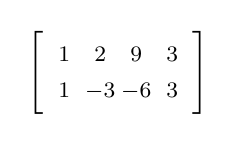
\begin{tikzpicture}[baseline={($(m-1-1)!.5!(m-2-1)$)}]
    \matrix (m)[tikz matrix]{
      1 & 2  & 9  & 3 \\
      1 & -3 & -6 & 3 \\
    };
  \end{tikzpicture}
\end{equation*}
\begin{equation*}
  M =
  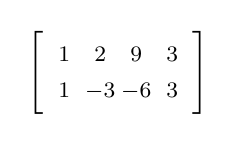
\begin{tikzpicture}[baseline={([yshift=-.5ex]$(m-1-1)!.5!(m-2-1)$)}]
    \matrix (m)[tikz matrix]{
      1 & 2  & 9  & 3 \\
      1 & -3 & -6 & 3 \\
    };
  \end{tikzpicture}
\end{equation*}
\end{document}